\subsection{Hardware Device}

\subsubsection{Block diagram}

The block diagram shown in \autoref{fig:block_diagram_hardware} provides an overview of the complete \gls{NEST} hardware architecture. It illustrates how the ESP32 microcontroller acts as the central hub, interacting with the sensing layer (DHT22, Load Cell, and \gls{RFID}) and the actuation layer (Servos and \gls{RGB} \gls{LED}). Each peripheral is connected through specialized interfaces, allowing the system to process data at the edge and perform autonomous egg protection tasks.

\begin{figure}[H]
    \centering
    \includegraphics[height=0.65\linewidth, angle=270]{images/block_diagram.png}
    \caption{Block Diagram of the Hardware System}
    \label{fig:block_diagram_hardware}
\end{figure}

The ESP32 microcontroller manages the diverse hardware modules. A digital interface is used to gather periodic temperature and humidity data from the DHT22. The \gls{SPI} bus is dedicated to the MFRC522 module for high-speed \gls{RFID} communication to identify hens and farmers. Weight data is acquired through a serial interface with the HX711 amplifier, while \gls{PWM} channels drive the SG90 servomotors for precise door positioning.

In addition, several \gls{GPIO} pins drive the \gls{RGB} \gls{LED} to provide immediate visual feedback on the system's state. The hardware configuration utilizes the ESP32's 3.3V and Arduino's 5V power supplies. Finally, all the data collected from the sensors is sent to the ThingsBoard server via \gls{MQTT} over a Wi-Fi connection, enabling remote monitoring and processing.

\subsubsection{Hardware Components}

\begin{itemize}
    \item \textbf{ESP32 Microcontroller\cite{ESP32WiFiBluetooth}}: The ESP32 is a high-performance \gls{SoC} featuring dual-core processors and integrated Wi-Fi connectivity. In the \gls{NEST} project, it is responsible for data acquisition from sensors, actuator Control and communication via \gls{MQTT}.

    \item \textbf{5 kg Weight Scale\cite{LoadCell} and HX711 Amplifier\cite{LoadCellAmplifier}}: For egg detection, a Load Cell is integrated with an HX711 24-bit \gls{ADC} amplifier. This allows the system to detect the presence and quantity of eggs by weight.
    
    Physically, the load cell operates as a transducer that converts mechanical force into an electrical signal. It contains an internal \textbf{Wheatstone bridge} of strain gauges: When a weight is placed on the platform, the resistance of these gauges changes, producing a differential voltage in the millivolt range. 

    Because this signal is too small for the ESP32 to process directly, the \textbf{HX711 amplifier} is used to amplify the signal and convert it into a 24-bit digital value. The HX711 connects to the ESP32 through \gls{GPIO} 16 (DOUT) and \gls{GPIO} 4 (SCK) using a two-wire serial interface. 

    \begin{figure}[H]
        \centering
        \includegraphics[width=1\textwidth]{images/circuit.png}
        \caption{Load Cell Diagram\cite{santosESP32LoadCell2022a}}
        \label{fig:load_cell_circuit}
    \end{figure}

    \clearpage

    \item \textbf{DHT22 Temperature and Humidity Sensor\cite{DHT22TemperatureHumidity}}: To monitor the incubation environment, the system integrates a DHT22 digital sensor. This sensor provides periodic measurements of ambient conditions, which are critical for egg quality monitoring. It communicates with the ESP32 via \gls{GPIO} 15 using a digital single-wire protocol.
    
    \begin{figure}[H]
        \centering
        \includegraphics[width=0.3\textwidth]{images/DHT22.png}
        \caption{DHT22 Circuit}
        \label{fig:dht22_circuit}
    \end{figure}

    \item \textbf{MFRC522 \gls{RFID} Module\cite{MODULORFIDRC522KIT}}: To handle hen detection, access control and identification, the system integrates an MFRC522 \gls{RFID} reader. It communicates with the ESP32 via the \gls{SPI} protocol using \gls{GPIO} pins 18 (SCK), 19 (MISO), 23 (MOSI), and 5 (SS).

    \item \textbf{SG90-180 Servo Motors\cite{MICROSERVOSG90180ºa}}: The physical response of the system is managed by two SG90-180 micro servo motors acting as actuators. These motors are responsible for open and close the doors of the nest. The ESP32 controls these servos using \gls{PWM} signals through \gls{GPIO} 2 and \gls{GPIO} 13. The use of actuators that can be triggered both by edge decisions and by remote commands.

    \item \textbf{\gls{RGB} \gls{LED} and 470 Ohm Resistors}: The system includes a common-anode \gls{RGB} \gls{LED} to provide local status indication. This \gls{LED} is controlled via \gls{GPIO} 25, 26, and 27. Each channel is connected in series with a 470 Ohm resistor to protect the ESP32 pins from overcurrent.

    \begin{figure}[H]
        \centering
        \includegraphics[width=0.3\textwidth]{images/RGB_circuit.png}
        \caption{\acrshort{RGB} \acrshort{LED} Circuit}
        \label{fig:rgb_circuit}
    \end{figure}

    \item \textbf{Arduino Microcontroller (Power Supply)}: Although the ESP32 acts as the central intelligence unit, an Arduino board has been integrated into the hardware architecture to function as a specialized power distribution bridge. The SG90 servo motors require a stable 5V supply to operate correctly under load. Since the ESP32 development board typically operates at 3.3V and its output pins cannot provide the necessary current or voltage for the actuators, the Arduino is utilized to leverage its 5V power rail.

\end{itemize}

\subsubsection{Interfaces of the system}

To ensure the reliability and modularity of the \gls{NEST} platform, the hardware architecture is organized into distinct electrical domains. The following tables detail the pin-mapping for logic signals, the power distribution strategy, and the specific wiring for high-precision sensing.

The integration utilizes diverse communication protocols, including \textbf{Single-Bus} for environmental data, \textbf{\gls{SPI}} for high-speed \gls{RFID} identification, and \textbf{\gls{PWM}} for precise mechanical control of the actuators.

\begin{table}[H]
    \centering
    \caption{Main System Connections (ESP32)}
    \label{tab:esp32_connections}
    \footnotesize
    \begin{tabular}{p{0.18\textwidth}p{0.12\textwidth}p{0.12\textwidth}p{0.18\textwidth}}
        \toprule
        \textbf{Module} & \textbf{Pin Name} & \textbf{ESP32 Pin} & \textbf{Function/Protocol} \\
        \midrule

        \multirow{3}{*}{DHT22 Temp/Hum} 
            & VCC & 3.3V & Power Supply \\
            & Data & GPIO 15 & Digital Single-Bus \\
            & GND & GND & Ground Reference \\
        \midrule

        \multirow{4}{*}{HX711 Amplifier} 
            & VCC & 3.3V & Power Supply \\
            & DOUT & GPIO 16 & Serial Data Out \\
            & SCK & GPIO 4 & Serial Clock \\
            & GND & GND & Ground Reference \\
        \midrule

        \multirow{8}{*}{MFRC522 \gls{RFID}} 
            & VCC & 3.3V & Power Supply \\
            & SCK & GPIO 18 & \gls{SPI} Clock \\
            & MISO & GPIO 19 & \gls{SPI} Master In \\
            & MOSI & GPIO 23 & \gls{SPI} Master Out \\
            & SS & GPIO 5 & \gls{SPI} Slave Select \\
            & RST & GPIO 22 & Reset \\
            & GND & GND & Ground Reference \\
            & IRQ & -- & -- \\
        \midrule

        \multirow{3}{*}{SG90-180 Servos} 
            & Servo 1 & GPIO 2 & \gls{PWM} \\
            & Servo 2 & GPIO 13 & \gls{PWM} \\
            & GND & GND & Ground Reference \\
        \midrule

        \multirow{4}{*}{\gls{LED} \gls{RGB} (Anode)} 
            & Common & 3.3V & Power Supply \\
            & R + 470 Ohm & GPIO 25 & Red \\
            & G + 470 Ohm & GPIO 26 & Green \\
            & B + 470 Ohm & GPIO 27 & Blue \\
        \bottomrule
    \end{tabular}
\end{table}

A critical aspect of the design is the \textbf{Power Decoupling} strategy. To prevent electrical noise and voltage drops caused by the SG90 servomotors from affecting the ESP32's logic, an Arduino board is used as a dedicated 5V power rail, sharing a common ground to maintain signal integrity.

\begin{table}[H]
    \centering
    \caption{Arduino Connections}
    \label{tab:arduino_power}
    \footnotesize
    \begin{tabular}{p{0.12\textwidth}p{0.12\textwidth}p{0.12\textwidth}p{0.25\textwidth}}
        \toprule
        \textbf{Device} & \textbf{Connection} & \textbf{Arduino Pin} & \textbf{Description} \\
        \midrule
        SG90 Servos & VCC & 5V & High Current Power Supply \\
        ESP32 & GND & GND & Ground Reference Unification \\
        \bottomrule
    \end{tabular}
\end{table}

For the production monitoring subsystem, the load cell is wired in a \textbf{Wheatstone Bridge} configuration. This setup allows the HX711 to detect minute changes in resistance and amplify them into 24-bit digital values for the ESP32.

\begin{table}[H]
    \centering
    \caption{Load Cell Wiring (Wheatstone Bridge)}
    \label{tab:load_cell_wiring}
    \footnotesize
    \begin{tabular}{p{0.12\textwidth}p{0.12\textwidth}p{0.12\textwidth}p{0.25\textwidth}}
        \toprule
        \textbf{Wire Color} & \textbf{Signal Type} & \textbf{HX711 Pin} & \textbf{Description} \\
        \midrule
        Red & Excitation+ & E+ & Positive Voltage Supply \\
        Black & Excitation- & E- & Negative Voltage Supply \\
        Green & Signal+ & A+ & Differential Output Positive \\
        White & Signal- & A- & Differential Output Negative \\
        \bottomrule
    \end{tabular}
\end{table}

\clearpage

\subsubsection{Final Prototype}

The final prototype integrates all previous modules into a compact hardware unit, as shown in \autoref{fig:prototype_photo}. This assembly was designed to withstand the environmental conditions of a farm while maintaining high precision in identifying individual hens and measuring egg production.

\begin{figure}[H]
    \centering
    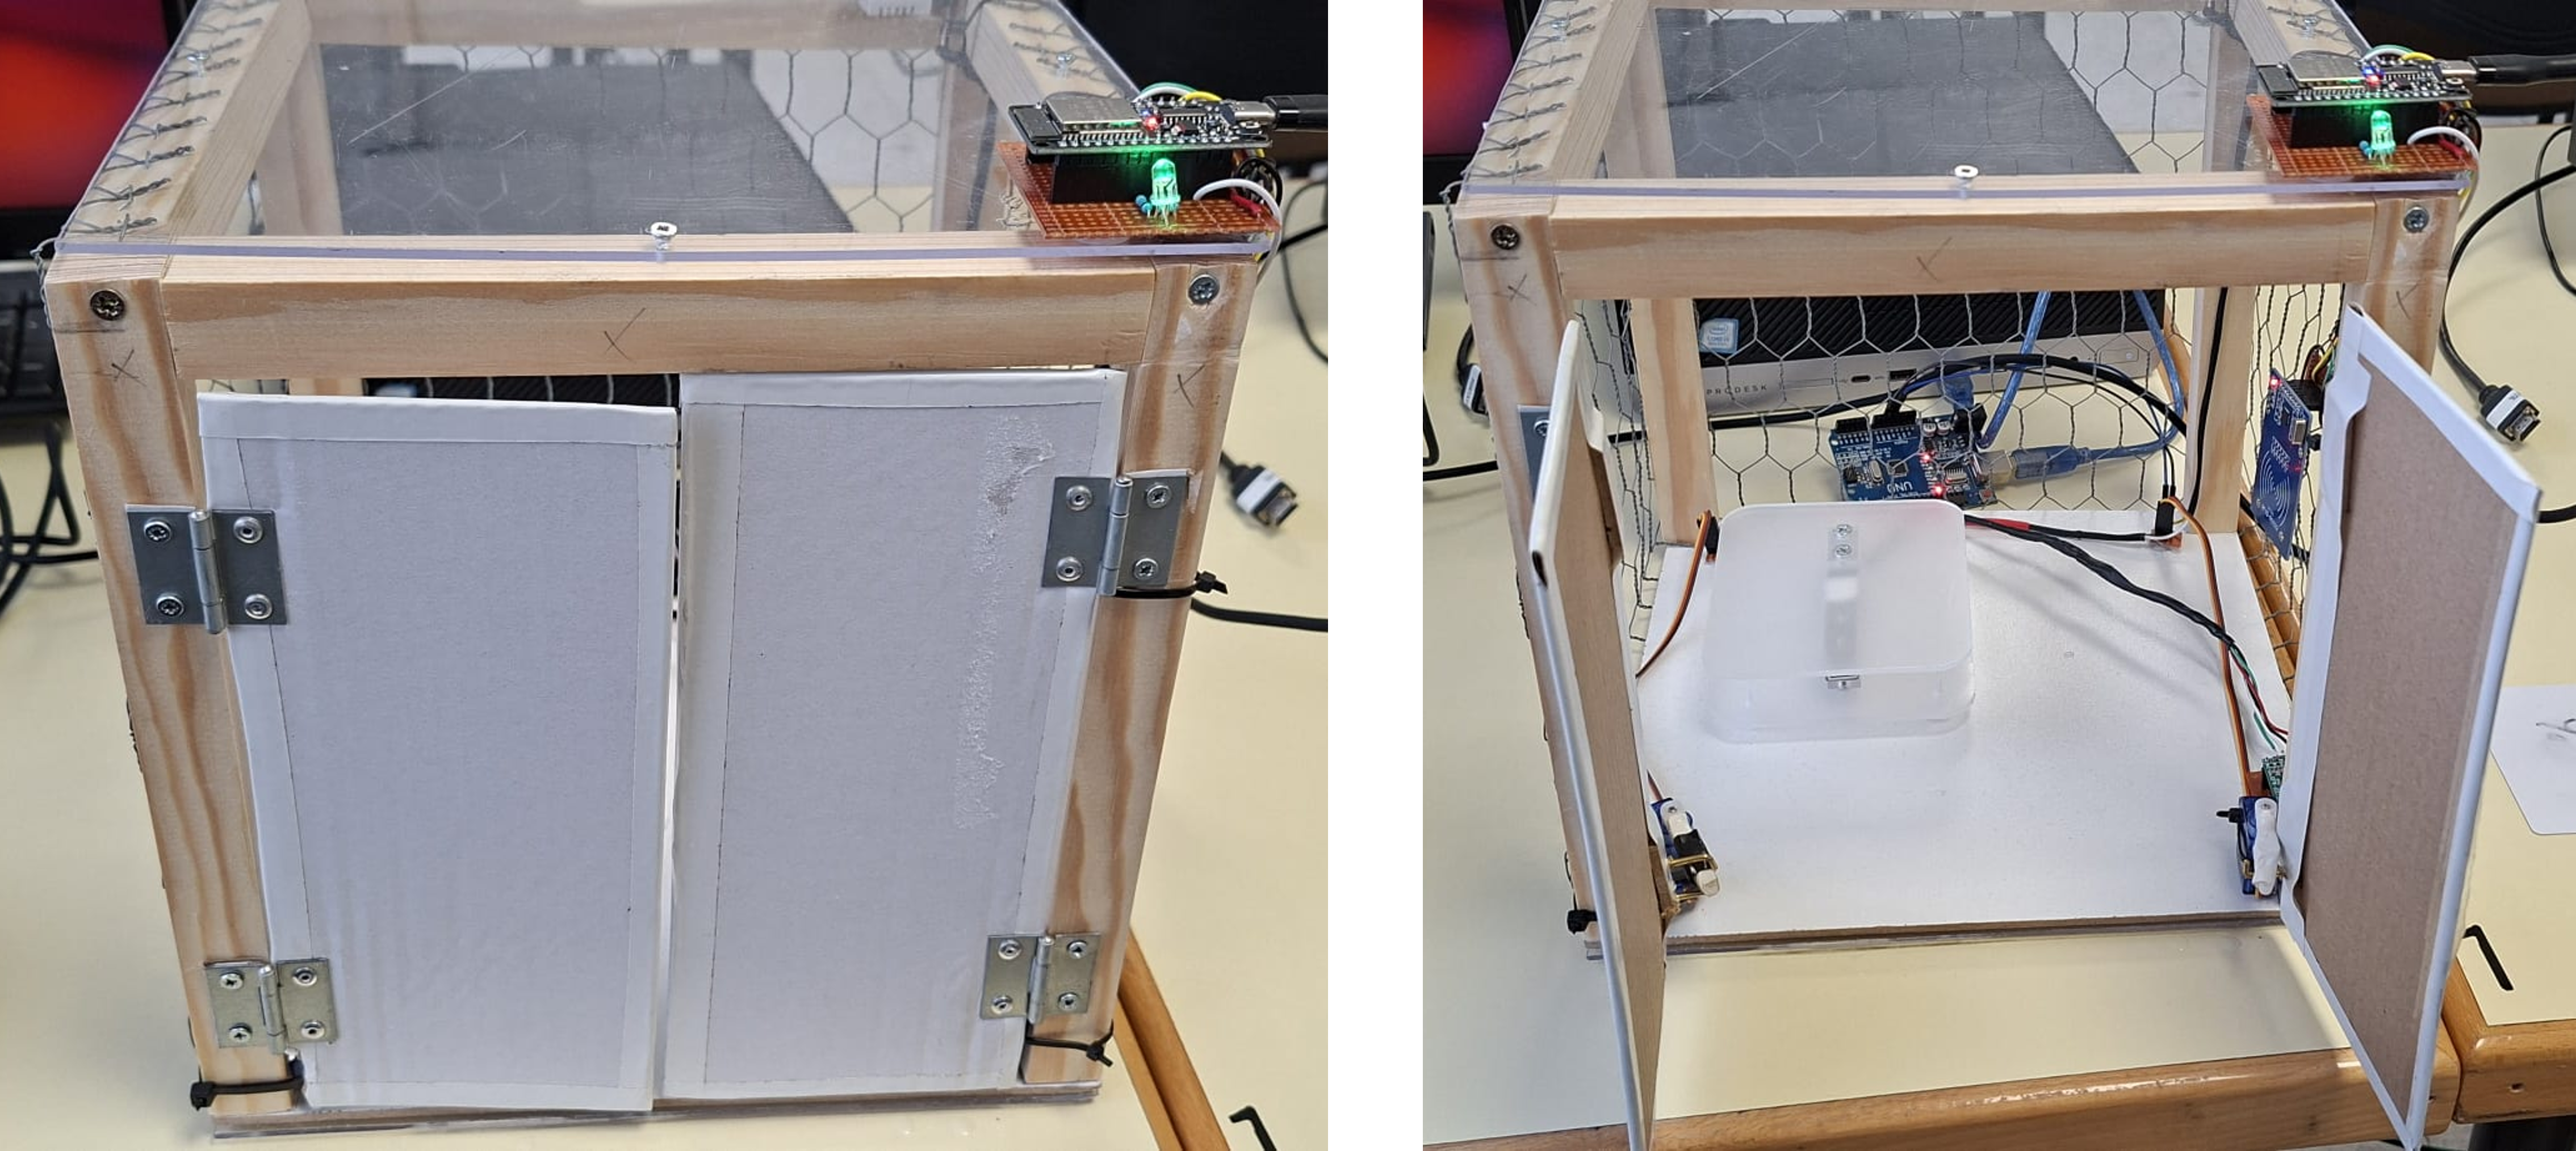
\includegraphics[width=0.5\textwidth]{images/hardware.jpeg}
    \caption{Final Prototype}
    \label{fig:prototype_photo}
\end{figure}

\begin{table}[H] 
    \centering 
    \caption{Hardware Specifications and Components} 
    \label{tab:hardware_specs} 
    \begin{tabular}{p{0.2\textwidth}p{0.63\textwidth}}
        \toprule
        \textbf{Component} & \textbf{Function} \\
        \midrule
        ESP32 & Data acquisition, actuators control, and communication (\gls{MQTT}). \\ 
        DHT22 & Periodic temperature and humidity sensing \\ 
        Load Cell + HX711 & Egg detection via weight measurement \\ 
        MFRC522 (\gls{RFID}) & Hens location, access control and identification \\ 
        SG90-180 Servo & Actuator for automated nesting box closure \\ 
        \gls{RGB} \gls{LED} & Local visual status notification and actuator feedback \\ 
        Arduino & Secondary power distribution (5V) \\ 
        \bottomrule
    \end{tabular} 
\end{table}

\autoref{tab:hardware_budget} is a summary of the costs associated with each hardware component used in the \gls{NEST} system.

\begin{table}[H] 
    \centering 
    \caption{Hardware Budget and Costs} 
    \label{tab:hardware_budget} 
    \begin{tabular}{p{0.3\textwidth}p{0.15\textwidth}p{0.15\textwidth}p{0.18\textwidth}}
        \toprule
        \textbf{Component} & \textbf{Price (€)} & \textbf{Amount} & \textbf{Final Price (€)} \\
        \midrule
        ESP32 & 4.39 & 1 & 4.39 \\ 
        Load Cell + HX711 + Platform & 4.42 & 1 & 4.42 \\ 
        DHT22 & 1.48 & 1 & 1.48 \\ 
        MFRC522 (\gls{RFID}) & 1.27 & 1 & 1.27 \\ 
        SG90-180 Servo & 1.24 & 2 & 2.48 \\ 
        \gls{RGB} \gls{LED} & 0.07 & 1 & 0.07 \\ 
        470 Ohm Resistors & 0.01 & 3 & 0.03 \\ 
        Arduino & -- & 1 & -- \\
        Electrical Materials & 10 & -- & 10 \\
        Box Materials & 20 & -- & 20 \\
        \midrule
        \textbf{Total Price} & & & 44.14 \\
        \bottomrule
    \end{tabular} 
\end{table}